% NeurIPS 2023 Paper Template
\documentclass{article}
\usepackage[final]{neurips_2023}

\usepackage[utf8]{inputenc} % allow utf-8 input
\usepackage[T1]{fontenc}    % use 8-bit T1 fonts
\usepackage{hyperref}       % hyperlinks
\usepackage{url}            % simple URL typesetting
\usepackage{booktabs}       % professional-quality tables
\usepackage{amsfonts}       % blackboard math symbols
\usepackage{nicefrac}       % compact symbols for 1/2, etc.
\usepackage{microtype}      % microtypography
\usepackage{xcolor}         % colors
\usepackage{authblk}
\usepackage{graphicx}
\usepackage{lipsum}         % for filler text if needed

\title{Privacy Ranker: Assessing Privacy Risk in Social Media Profiles}

\author[1]{Justin Hoyle}
\author[2]{Matthew Glennon}
\author[3]{Jay Darshitbhai Patel}

\affil[1,2,3]{Virginia Commonwealth University}
\affil[1]{\texttt{hoylejb2@vcu.edu}}
\affil[2]{\texttt{mglennon@vcu.edu}}
\affil[3]{\texttt{patelj33@vcu.edu}}

\begin{document}

\maketitle

\begin{abstract}
This project aims to develop a Privacy Ranker that evaluates and ranks users’ social media profiles based on their privacy risk. Many users unknowingly expose Personally Identifiable Information (PII) on platforms such as Twitter, LinkedIn, and Instagram, leading to privacy leaks, identity theft, and more. Our approach leverages a combination of natural language processing and machine learning techniques to extract PII from raw textual data and to assess the associated privacy risk.
\end{abstract}

\section{Introduction}
In today's digital era, social media platforms are ubiquitous channels for communication and self-expression. However, the ease of sharing information often leads to unintended exposure of sensitive data. This exposure can increase the risk of identity theft, phishing, and unauthorized data aggregation. Our project addresses these challenges by developing a system—the \emph{Privacy Ranker}—that automatically identifies PII in social media posts and assigns a privacy risk score based on the volume and type of exposed information.

\section{Data Source}
The primary dataset used in this project is the Sentiment140 dataset (\url{https://www.kaggle.com/datasets/kazanova/sentiment140}), originally designed for sentiment analysis. Despite its original purpose, the rich textual content of tweets makes this dataset an excellent candidate for evaluating privacy risks. To tailor the dataset for our analysis, additional annotations have been introduced to label and highlight PII, which serve as inputs for subsequent processing stages.

\section{Methodology}
The overall pipeline of the Privacy Ranker comprises several key stages. Each stage is implemented in separate Python scripts, as described below.

\subsection{Data Cleaning}
Data cleaning is implemented in \texttt{clean\_csv.py}. The process consists of:
\begin{itemize}
    \item \textbf{CSV Parsing:} The dataset is read using \texttt{pandas} with the proper encoding (``latin-1'').
    \item \textbf{Column Reduction:} The raw CSV file contains several columns; the script drops columns with indices 0, 2, and 3, retaining only the tweet ID, user identifier, and tweet text.
    \item \textbf{Data Quality Assurance:} After renaming the remaining columns to \texttt{ids}, \texttt{user}, and \texttt{text}, empty entries and duplicate tweets are removed.
    \item \textbf{Text Cleaning:} A custom function \texttt{clean\_text()} converts text to lowercase and uses regular expressions to strip URLs, mentions, hashtags, punctuation, and common stopwords (via NLTK).
\end{itemize}

\subsection{Computational Infrastructure}
All model training and evaluation tasks were performed using the Apollo cluster at the Virginia Commonwealth University (VCU) High Performance Research Computing (HPRC) facility. Apollo is designed to support research using data requiring compliance with federal security and privacy standards. It consists of 18 compute nodes, 604 CPUs, 5.9 TB of RAM, 3 PB of high-performance Lustre file system storage, and Nvidia P100 GPUs connected via 54 Gb/second InfiniBand networking. This secure and robust computing environment enabled the efficient training of transformer-based models, including DistilBERT, on large text datasets.

\subsection{Named Entity Recognition for PII Extraction}
The extraction of PII is implemented in \texttt{named\_entity\_recognition.py} using Hugging Face's \texttt{transformers} library. Specifically, the script leverages the \texttt{Jean-Baptiste/roberta-large-ner-english} model and its associated tokenizer to create a NER pipeline. This pipeline, which utilizes GPU acceleration when available, processes text to identify entities such as \texttt{PER}, \texttt{ORG}, \texttt{LOC}, and \texttt{MISC}. In addition, regular expressions are applied to capture emails and phone numbers. The results from the Hugging Face pipeline and regex matching are combined into a single output per tweet.

\subsection{Feature Engineering and Machine Learning}
Two modeling approaches are implemented in this project. The first is a classical machine learning pipeline using a Random Forest classifier. In this approach, features are engineered by combining TF-IDF vectorization of the raw text with structured features such as the presence of PII entities (e.g., \texttt{has\_person}, \texttt{has\_org}, \texttt{has\_gpe}), text length, and word count. The Random Forest model is trained on these concatenated features after addressing class imbalance with SMOTE.

\subsubsection{Transformer-Based Model (DistilBERT)}
In addition, a transformer-based model using DistilBERT is implemented in \texttt{feature\_processing.py}. This approach involves tokenizing the text data, preparing datasets using Hugging Face's \texttt{Dataset} library, and training a sequence classification model with Hugging Face’s \texttt{Trainer}. The training process includes dataset preparation, tokenization, and evaluation using accuracy metrics. The final model is saved for future inference.

\subsection{Model Training and Evaluation}
The Random Forest model, as configured in \texttt{feature\_processing.py}, is trained on the oversampled training data. Evaluation is performed using:
\begin{itemize}
    \item \textbf{Classification Report:} Metrics such as precision, recall, and F1-score are calculated to assess model performance.
    \item \textbf{Confusion Matrix:} This provides a visual insight into the classification accuracy across different risk levels.
\end{itemize}
Once evaluated, the trained model and the TF-IDF vectorizer are persisted using \texttt{joblib}, making them available for future predictions.

\subsection{Model Testing}
A separate script, \texttt{test\_model.py}, is responsible for loading the saved Random Forest model and TF-IDF vectorizer. The script applies the same preprocessing steps as used during training to prepare new data, and then demonstrates inference by predicting privacy risk labels. Additionally, it evaluates the model's performance using a classification report that summarizes precision, recall, and F1-score.

\section{Experimental Setup and Results}
The experiments were conducted on a standard workstation. Key aspects include:
\begin{itemize}
    \item \textbf{Data Sampling:} To maintain computational efficiency, only 10\% of unique users from the dataset were included.
    \item \textbf{Train-Test Split:} An 80/20 split was employed to create the training and test sets.
    \item \textbf{Oversampling:} SMOTE was applied to the training data to balance the distribution of risk labels.
    \item \textbf{Model Configuration:} The Random Forest classifier was configured with a maximum depth of 20, 200 estimators, and balanced class weights.
\end{itemize}

\begin{figure}[ht]
    \centering
    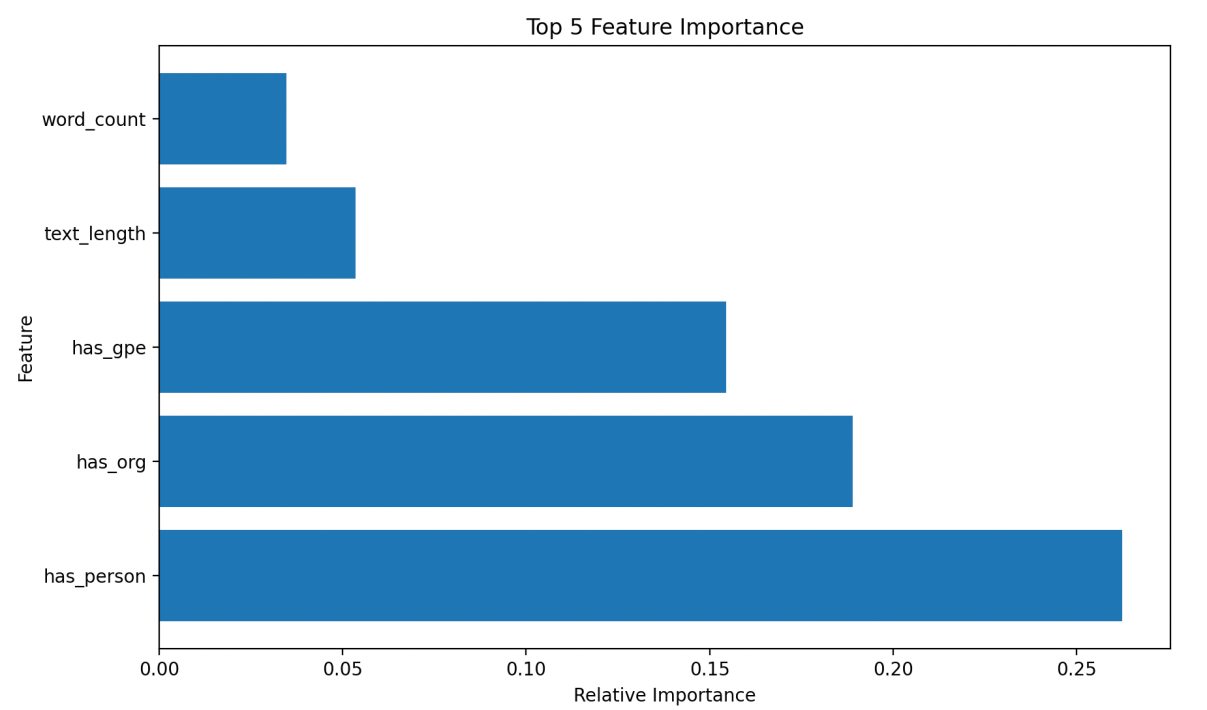
\includegraphics[width=0.6\linewidth]{fi.png}
    \caption{Top 5 Feature Importance in the Random Forest Classifier.}
    \label{fig:feature_importance}
\end{figure}

\begin{figure}[ht]
    \centering
    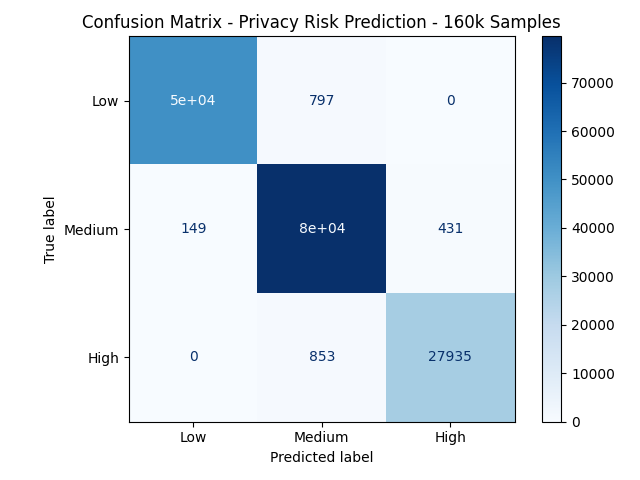
\includegraphics[width=0.6\linewidth]{cm.png}
    \caption{Confusion matrix for the Random Forest classifier on the test set.}
    \label{fig:confusion}
\end{figure}

Figure \ref{fig:feature_importance} shows that the presence of a \texttt{PERSON} entity (\texttt{has\_person}) is the most significant contributor to the model’s decision-making process, followed by \texttt{has\_org}, \texttt{has\_gpe}, and text-based metrics such as \texttt{text\_length} and \texttt{word\_count}.

After training and evaluation, we generated a confusion matrix to visualize the classification performance. Figure \ref{fig:confusion} presents the true versus predicted risk labels.

\section{Discussion}
Our implementation demonstrates a systematic approach to privacy risk assessment:
\begin{itemize}
    \item The dual approach for PII extraction—combining spaCy's transformer-based NER with regular expressions—ensures that a wide variety of PII is captured.
    \item Data cleaning and preprocessing steps are essential to reduce noise and improve the quality of input data.
    \item Feature engineering, which includes both text-based features and structured indicators, provides a comprehensive representation of the data.
    \item The use of SMOTE to mitigate class imbalance significantly contributes to the robustness of the trained Random Forest classifier.
\end{itemize}
The modular design, with distinct scripts for cleaning, extraction, feature processing, and model testing, facilitates easier debugging and future enhancements.

\section{Conclusion and Future Work}
This paper presented an end-to-end framework for assessing privacy risks in social media profiles by detecting and classifying PII. The Privacy Ranker system integrates robust data preprocessing, advanced PII extraction using Hugging Face’s transformers, comprehensive feature engineering, and both classical and transformer-based machine learning approaches to generate actionable risk scores.

Future work may include:
\begin{itemize}
    \item Integrating more advanced deep learning models for both text representation and risk prediction.
    \item Expanding the dataset to include additional social media platforms and non-English languages.
    \item Conducting user studies to further validate the practical utility of the Privacy Ranker in real-world scenarios.
    \item Exploring the adaptability of the system to various deployment constraints by leveraging multiple modeling paradigms.
\end{itemize}
Overall, our work demonstrates the potential of combining classical machine learning and transformer-based approaches to create a flexible and robust privacy risk assessment tool.

\section{Code Repository}
The complete codebase for this project is available at:
\url{https://github.com/JustinHoyle/Final-Project-CMSC-512}

The repository includes:
\begin{itemize}
    \item \texttt{clean\_csv.py}: Implements CSV parsing, text cleaning, and removal of irrelevant mentions.
    \item \texttt{named\_entity\_recognition.py}: Extracts PII using both spaCy NER and regex patterns.
    \item \texttt{feature\_processing.py}: Handles feature engineering, TF-IDF vectorization, model training, and evaluation.
    \item \texttt{test\_model.py}: Demonstrates how to load the trained model and vectorizer to predict privacy risk on new data.
    \item Additional scripts and notebooks for exploratory data analysis.
\end{itemize}

\section{Acknowledgements}
We would like to thank our advisors and colleagues at Virginia Commonwealth University for their invaluable support and feedback throughout this project.

\section*{References}
\begin{itemize}
    \item \texttt{pandas} documentation: \url{https://pandas.pydata.org/}
    \item \texttt{nltk} documentation: \url{https://www.nltk.org/}
    \item \texttt{spaCy} documentation: \url{https://spacy.io/}
    \item \texttt{scikit-learn} documentation: \url{https://scikit-learn.org/}
    \item \texttt{imbalanced-learn} (SMOTE): \url{https://imbalanced-learn.org/}
\end{itemize}

\end{document}